\graphicspath{ {04-TransferMatrices/Figures/} }

\section{Transfer matrices}

A beam line may be described as a series of beam-line elements
arranged one after the other.
A particle may then be transported through the beam line by
transporting it through each element in turn.
Taking advantage of the trace-space defined above, the transport of
a particle across a particular beam-line element may be performed
using a linear transformation:
\begin{equation}
  \underline{\phi}_{\rm\,end} = \underline{\underline{T}} ~
                            \underline{\phi}_{\rm\,start} \, ;
\end{equation}
where $\underline{\phi}_{\rm\,start}$ is the trace-space vector at the
start of the beam-line element and $\underline{\phi}_{\rm\,end}$ is
the transformed trace-space vector at the end.
The step across the beam-line element implies an increment, $\delta s$,
to the $s$-coordinate given by:
\begin{equation}
  s_{\rm end} = s_{\rm start} + \delta s \, ;
\end{equation}
where $s_{\rm start}$ and $s_{\rm end}$ are the coordinate along the
reference particle trajectory at the start and end of the beam-line
element respectively.
Equation~\ref{Eq:Cov6} implies that the covariance matrix may be
transported across a beam-line element using the expression:
\begin{equation}
  \underline{\underline{C}}_{6\,\rm end} =
     \underline{\underline{T}}~
       \underline{\underline{C}}_{6\,\rm start}~
     \underline{\underline{T}}^T \, .
\end{equation}

There are many excellent descriptions of the derivation of the
transfer matrices, $\underline{\underline{T}}$, so only the results
are quoted here.
The notation used below is developed from that used
in~\cite{Wolski:2014}.

\subsection{Drift}

A ``drift'' space refers to a region in which the beam propagates in
the absence of any electromagnetic fields.
In a drift, particles propagate in straight lines, therefore:
\begin{equation}
  \underline{\underline{T}}_{\rm~drift} =
        \begin{pmatrix}
          1 & l & 0 & 0 & 0 &                             0 \\
          0 & 1 & 0 & 0 & 0 &                             0 \\
          0 & 0 & 1 & l & 0 &                             0 \\
          0 & 0 & 0 & 1 & 0 &                             0 \\
          0 & 0 & 0 & 0 & 1 & \frac{l}{\beta_0^2 \gamma_0^2} \\
          0 & 0 & 0 & 0 & 0 &                             1
        \end{pmatrix} \, ; 
\end{equation}
where $l$ is the length of the drift.
The increment in the reference particle position is:
\begin{equation}
  \delta s = l \, .
\end{equation}

\subsection{Quadrupole}

The passage of a beam particle through a quadrupole magnet may be
described by specifying the field gradient, $g$, within the magnet and
the length, $l_q$, of the quadrupole measured along its axis.
The impact of a quadrupole on the trajectory of a particle in the $xy$
plane is independent of the impact of the magnet on the particle's
trajectory in the $yz$ plane.   
In this sense quadrupole focusing in the $xz$ and $yz$ planes is said
to be ``uncoupled''. 

If the field gradient along the $x$ and $y$ axes is identical, then:
\begin{equation}
  g_x = \frac{\partial B_{qx}}{\partial x} =
  g_y = \frac{\partial B_{qy}}{\partial y} = g \, ; \label{Eq:Trnsf:gxy}
\end{equation}
where the field in the quadrupole, $\bm{B_q}$, has components
$(B_{qx}, B_{qy}, 0)$.

In the ``hard-edge'' approximation, where the field falls to zero at
the start and end of the quadrupole, the transfer matrix for a
quadrupole focusing in the $xz$ plane (a ``focusing quadrupole'') may
be written: 
\begin{equation}
  \underline{\underline{T}}_{\rm~Fquad} =
    \begin{pmatrix}
          \cos(\sqrt{k_q} l_q) & \frac{\sin(\sqrt{k_q} l_q)}{\sqrt{k_q}} & 0 & 0             & 0 & 0 \\
-\sqrt{k_q} \sin(\sqrt{k_q} l_q) &                  \cos(\sqrt{k_q} l_q) & 0 & 0             & 0 & 0 \\
          0 & 0 &           \cosh(\sqrt{k_q} l_q) & \frac{\sinh(\sqrt{k_q} l_q)}{\sqrt{k_q}} & 0 & 0 \\
          0 & 0 &  \sqrt{k_q} \sinh(\sqrt{k_q} l_q) &                  \cosh(\sqrt{k_q} l_q) & 0 & 0 \\
          0 & 0 & 0 & 0 & 1 & \frac{l_q}{\beta_0^2 \gamma_0^2} \\
          0 & 0 & 0 & 0 & 0 &                             1
        \end{pmatrix} \, ; 
\end{equation}
where:
\begin{equation}
  k_q = \frac{gc}{p} \times 10^{-3} \, {\rm m}^{-2} \, ,
                                                   \label{Eq:Effectivekq}
\end{equation}
$c$ is the speed of light in metres per second, $p$ is the magnitude
of the momentum of the particle in MeV/c, and the field gradient, $g$,
is given in T/m. 
As before, $\beta_0$ is the relativistic velocity of the reference
particle and $\gamma_0=(1-\beta_0^2)^{-\frac{1}{2}}$.
The increment in the reference particle position is:
\begin{equation}
  \delta s = l_q \, .
\end{equation}

It is important to include a description of the effect of dispersion
on beam transport through the LhARA beam line since the laser-driven
proton and ion source provides a broad energy spectrum. 
Reference \cite{Wolski:2014} describes two methods for the description
of dispersion in a linear approximation.
The first is to use the reference momentum to calculate the quadrupole
focusing strength ($k_{0q} = \frac{gc}{p_0} \times 10^{-3}$\,m$^{-2}$)
and to include terms in the expressions for $x$, $x^\prime$, $y$, and
$y^\prime$ dependent on $\delta$.    
The second is to use equation~\ref{Eq:Effectivekq} to calculate the
effective quadrupole focusing strength, with $k_q$ evaluated using
$p$.
The second approach has been adopted here.

In the same notation, the transfer matrix for a quadrupole focusing in
the $yz$ plane (a ``defocusing quadrupole'') may be written: 
\begin{equation}
  \underline{\underline{T}}_{\rm~Dquad} =
    \begin{pmatrix}
          \cosh(\sqrt{k_q} l_q) & \frac{\sinh(\sqrt{k_q} l_q)}{\sqrt{k_q}} & 0 & 0             & 0 & 0 \\
 \sqrt{k_q} \sinh(\sqrt{k_q} l_q) &                  \cosh(\sqrt{k_q} l_q) & 0 & 0             & 0 & 0 \\
          0 & 0 &            \cos(\sqrt{k_q} l_q) &  \frac{\sin(\sqrt{k_q} l_q)}{\sqrt{k_q}} & 0 & 0 \\
          0 & 0 &  -\sqrt{k_q} \sin(\sqrt{k_q} l_q) &                   \cos(\sqrt{k_q} l_q) & 0 & 0 \\
          0 & 0 & 0 & 0 & 1 & \frac{l_q}{\beta_0^2 \gamma_0^2} \\
          0 & 0 & 0 & 0 & 0 &                             1
        \end{pmatrix} \, .
\end{equation}

\subsection{Solenoid}

The trajectory of a beam particle through a solenoid is determined by
the magnetic field strength, $\bm{B}_s$, within the solenoid and the
length of the solenoid, $l_s$, measured along its axis.
As the particle enters the solenoid, the fringe field imparts momentum
transverse to the axis of the magnet.
This results in the particle executing a helical trajectory, the axis
of the helix being parallel to the solenoid axis.
The sense of the rotation depends on the particle charge and the
polarity of the field.
The helical motion means that the evolution of the particle motion in
the $xz$ plane is coupled with the evolution of the particle motion in
the $yz$ plane.

In the ``hard-edge'' approximation, the magnetic field inside the
magnet is given by $\bm{B}_s = (0, 0, B_{s0})$, where the solenoid axis
lies along the $z_{\rm RPLC}$ axis.
The solenoid field-strength parameter is then given by:
\begin{equation}
  k_s = \left[ \frac{B_{s0} c}{2p} \times 10^{-3} \right]^2 \, {\rm m}^{-2}\,;
  \label{Eq:Effectiveks}
\end{equation}
where $B_{s0}$ is measured in T, $p$ in MeV/c and $c$ in m/s.

The transfer matrix for passage of a positive particle through a
solenoid with field pointing in the positive $z_{\rm RPLC}$ direction
may be written: 
\begin{equation}
  \underline{\underline{T}}_{\rm~Sol} =
    \begin{pmatrix}
                           \cos^2(\sqrt{k_s} l_s) &   \frac{1}{2\sqrt{k_s}} \sin(\sqrt{k_s} l_s) &           \frac{1}{2} \sin(2\sqrt{k_s} l_s) & \frac{1}{\sqrt{k_s}} \sin^2(\sqrt{k_s} l_s) & 0 & 0 \\
      -\frac{\sqrt{k_s}}{2} \sin(2\sqrt{k_s} l_s) &                       \cos^2(\sqrt{k_s} l_s) &           -\sqrt{k_s}\sin^2(\sqrt{k_s} l_s) &           \frac{1}{2} \sin(2\sqrt{k_s} l_s) & 0 & 0 \\
               -\frac{1}{2} \sin(2\sqrt{k_s} l_s) & -\frac{1}{\sqrt{k_s}} \sin^2(\sqrt{k_s} l_s) &                      \cos^2(\sqrt{k_s} l_s) & \frac{1}{2\sqrt{k_s}} \sin(2\sqrt{k_s} l_s) & 0 & 0 \\
                \sqrt{k_s} \sin^2(\sqrt{k_s} l_s) &           -\frac{1}{2} \sin(2\sqrt{k_s} l_s) & -\frac{\sqrt{k_s}}{2} \sin(2\sqrt{k_s} l_s) &                      \cos^2(\sqrt{k_s} l_s) & 0 & 0 \\
          0 & 0 & 0 & 0 & 1 & \frac{l}{\beta_0^2 \gamma_0^2} \\
          0 & 0 & 0 & 0 & 0 &                             1
        \end{pmatrix} \, .
\end{equation}
As in the case of the quadrupoles, dispersion is accounted for by
using $p$ to calculate $k_s$ (equation~\ref{Eq:Effectiveks}).
The increment in the reference particle position is:
\begin{equation}
  \delta s = l_s \, .
\end{equation}

\subsection{Non-neutral (electron) plasma (Gabor) lens}
\label{SubSect:TrnsFrMtrx:GL}

A dense gas of electrons confined in a Penning-Malmberg trap provides
an electric field that can be used to focus a positive ion beam.
The electron gas is confined axially in the lens by an electrostatic 
potential created using a central anode of length $l_G$.
The gas is confined radially using the uniform field of a solenoid.
Assuming a uniform electron density, $n_e$, the focusing parameter,
$k_G$, may be written:
\begin{equation}
  k_G = \frac{e}{2\epsilon_0} \frac{m_p \gamma}{p^2} n_e
                              \quad {\rm m}^{-2}
                              \, ; \label{Eq:EffectivekG}
\end{equation}
where $e$ is the charge on the electron, $\epsilon_0$ is the
permittivity of free space, and $m_p$ is the proton mass.
As in the case of the quadrupoles and solenoid, dispersion is
accounted for by using $p$ in equation~\ref{Eq:EffectivekG}.
The force on a particle passing through the electron gas is towards
the axis of the lens and is proportional to the radial distance of the
particle from the axis.
Focusing is therefore cylindrically symmetric and does not couple
motion in the the $xz$ and $yz$ planes.

In the ``hard-edge'' approximation, the electric field inside the
lens falls to zero at the end of the electron gas and the contribution
of the magnetic field used to confine the electron gas in the
transverse direction has a negligible effect on particles passing
through the lens.
The transfer matrix for the passage of a positive particle through the
lens may be written: 
\begin{equation}
  \underline{\underline{T}}_{G} =
    \begin{pmatrix}
                    \cos(\sqrt{k_G} l_G) & \frac{\sin(\sqrt{k_G} l_G)}{\sqrt{k_G}} &  0 & 0 & 0 & 0 \\
        -\sqrt{k_G} \sin(\sqrt{k_G} l_G) &                    \cos(\sqrt{k_G} l_G) &  0 & 0 & 0 & 0 \\
                                     0 &                                     0 &              \cos(\sqrt{k_G} l_G) & \frac{\sin(\sqrt{k_G} l_G)}{\sqrt{k_G}}  & 0 & 0 \\
                                     0 &                                     0 &  -\sqrt{k_G} \sin(\sqrt{k_G} l_G) &                     \cos(\sqrt{k_G} l_G) & 0 & 0 \\
          0 & 0 & 0 & 0 & 1 & \frac{l}{\beta_0^2 \gamma_0^2} \\
          0 & 0 & 0 & 0 & 0 &                             1
        \end{pmatrix} \, .
\end{equation}
The increment in the reference particle position is:
\begin{equation}
  \delta s = l_G \, .
\end{equation}

\subsection{Dipole}

The reference particle trajectory in the beam-line elements described
above passes along the axis of the element.
In contrast, a dipole bends the reference trajectory so that it
describes the arc of a circle (see figure~\ref{fig:Dipole}).
The code provides for transport through a ``sector dipole'' in the
hard-edge approximation. 
In this case, the field within the magnet is taken to be constant and
parallel to $\bm{j}_{\rm RPLC}$, i.e. $\bm{B}_D = (0, B_{D0}, 0)$. 
No edge focusing is considered.
\begin{figure}
  \begin{center}
    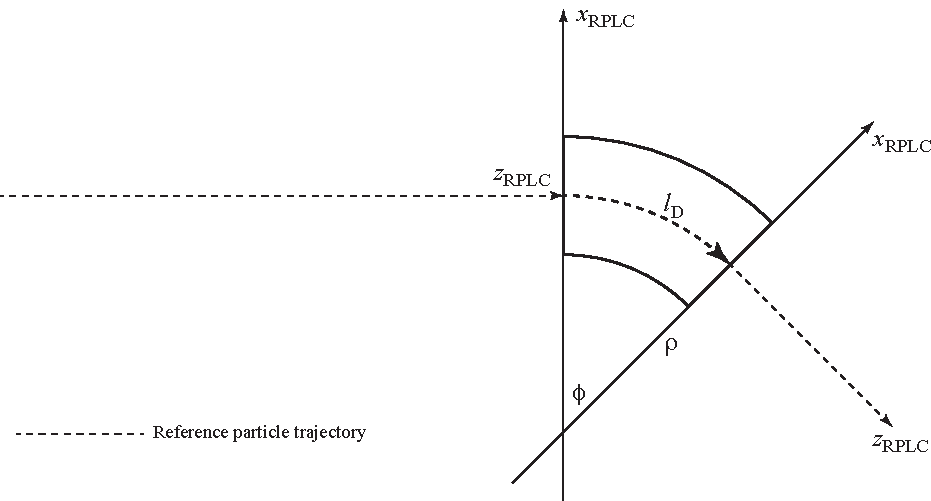
\includegraphics[width=0.85\textwidth]{Dipole.pdf}
  \end{center}
  \caption{
    Schematic representation of the passage of the reference particle
    through a sector dipole.
    The outline of the sector dipole is shown by the solid black
    lines.
    The trajectory of the reference particle is shown as the dashed
    line.
    The length of the reference-particle trajectory inside the field
    of the sector dipole is $l_D$.
    The $x_{\rm RPLC}$ and $z_{\rm RPLC}$ coordinate axes at the entry
    and exit of the sector dipole are shown.
    The radius of curvature of the reference particle trajectory
    inside the magnet is $\rho$ and the angle through which the
    $x_{\rm RPLC}$ is rotated is $\phi$. 
  }
  \label{fig:Dipole}
\end{figure}

The passage of particles through a dipole may be described by defining
the parameter, $k_D$:
\begin{equation}
  k_D = \left[ \frac{B_{D0} c}{p} \times 10^{-3} \right]^2\, {\rm m}^{-2} \, .
  \label{Eq:EffectivekD}
\end{equation}
The momentum of the reference particle is related to the
curvature. $\rho$, by:
\begin{equation}
  p_0 = B_{D0} \rho \, ;
\end{equation}
so:
\begin{equation}
  k_D = \frac{1}{\rho} \, ; 
\end{equation}
and the angle $\phi$ is given by:
\begin{equation}
  \phi = \frac{l_D}{\rho} \, .
\end{equation}
With these definitions the transfer matrix for passage through a
dipole may be written:
\begin{equation}
  \underline{\underline{T}}_{D} =
    \begin{pmatrix}
                    \cos(\phi) &                                  \rho \sin(\phi) & 0 & 0 & 0 &                 \frac{\rho}{\beta_0}\left(1 - \cos(\phi) \right) \\
      -\frac{\sin(\phi)}{\rho} &                                       \cos(\phi) & 0 & 0 & 0 &                                       \frac{\sin(\phi)}{\beta_0} \\
                             0 &                                                0 & 1 & l & 0 &                                                                0 \\
                             0 &                                                0 & 0 & 1 & 0 &                                                                0 \\
   -\frac{\sin(\phi)}{\beta_0} &  -\frac{\rho}{\beta_0}\left(1 -\cos(\phi)\right) & 0 & 0 & 1 & \frac{l}{\beta^2 \gamma^2} - \frac{l - \rho\sin(\phi)}{\beta_0^2} \\
                             0 &                                                0 & 0 & 0 & 0 &                                                                1
        \end{pmatrix} \, .
\end{equation}
The increment in the reference particle position is:
\begin{equation}
  \delta s = l_D \, .
\end{equation}
